%%%%%%%%%%%%%%%%%%%%%%%%%%%%%%%%%%%%%%%%%%%%%%%%%%%%%%%%%%%%%%%%%%%%%%%%%%%%%%%%%%%
%% This project aims to create the UFC template for presentation.                %%
%% author: Maurício Moreira Neto - Doctoral student in Computer Science (MDCC)   %%
%% contacts:                                                                     %%
%%    e-mail: maumneto@ufc.br                                                    %%
%%    linktree: https://linktr.ee/maumneto                                       %%
%%%%%%%%%%%%%%%%%%%%%%%%%%%%%%%%%%%%%%%%%%%%%%%%%%%%%%%%%%%%%%%%%%%%%%%%%%%%%%%%%%%
\documentclass{libs/ufc_format}
% Inserting the preamble file with the packages
%%%%%%%%%%%%%%%%%%%%%%%%%%%%%%%%%%%%%%%%%%%%%%%%%%%%%%%%%%%%%%%%%%%%%
%% This file contains the packages that can be used in the beamer. %%
%%%%%%%%%%%%%%%%%%%%%%%%%%%%%%%%%%%%%%%%%%%%%%%%%%%%%%%%%%%%%%%%%%%%%
% Package to fonts family
\usepackage[T1]{fontenc}
% Package to accentuation
\usepackage[utf8]{inputenc}
% Package to Portuguese language
\usepackage[brazil]{babel}
% Package to Figures
\usepackage{graphicx}
% Package to the colors
\usepackage{color}
% Package to the colors
\usepackage{xcolor}
% Packages to math symbols and expressions
\usepackage{amsfonts, amssymb, amsmath}
% Package to multiple lines and columns in table
\usepackage{multirow, array} 
% Package to create pseudo-code
% For more detail of this package: http://linorg.usp.br/CTAN/macros/latex/contrib/algorithm2e/doc/algorithm2e.pdf
\usepackage{algorithm2e}
% Package to insert code
\usepackage{listings} 
\usepackage{keyval}
% Package to justify text
\usepackage[document]{ragged2e}
% Package to manage the bibliography
\usepackage[backend=biber, style=numeric, sorting=none]{biblatex}
% Package to facilities quotations
\usepackage{csquotes}
% Package to use multicols
\usepackage{multicol}

% Packages added by me
\usepackage{url}
\usepackage{tikz}
%\usepackage{multimedia}
%\usepackage{media9}[playbutton=plain, windowed=1280x720]
% Inserting the references file
\bibliography{references.bib}
\renewcommand*{\bibfont}{\scriptsize}

% Title
\title[ML]{\huge\textbf{Redes de Computadores}}
% Subtitle
\subtitle{Parte 2}
% Author of the presentation
\author{Evandro J.R. Silva}
% Institute's Name
\institute[Estácio Teresina]{
    % email for contact
    \normalsize{\email{ejrs.profissional@gmail.com}}
    \newline
    % Department Name
    \department{Bacharelado em Ciência da Computação}
    \newline
    % university name
    %\ufc
    \estaciothe
}
% date of the presentation
\date{05 a 06 de Agosto}


%%%%%%%%%%%%%%%%%%%%%%%%%%%%%%%%%%%%%%%%%%%%%%%%%%%%%%%%%%%%%%%%%%%%%%%%%%%%%%%%%%
%% Start Document of the Presentation                                           %%               
%%%%%%%%%%%%%%%%%%%%%%%%%%%%%%%%%%%%%%%%%%%%%%%%%%%%%%%%%%%%%%%%%%%%%%%%%%%%%%%%%%
\begin{document}
% insert the code style
%%%%%%%%%%%%%%%%%%%%%%%%%%%%%%%%%%%%%%%%%%%%%%%%%%%%%%%%%%%%%%%%%%%%%%%%%%%%%%%%%%%
%% This file contains the style of the codes show in slides.                     %%
%% The package used is listings, but it possible to used others.                 %%
%%%%%%%%%%%%%%%%%%%%%%%%%%%%%%%%%%%%%%%%%%%%%%%%%%%%%%%%%%%%%%%%%%%%%%%%%%%%%%%%%%%

% color used in the code style
\definecolor{codegreen}{rgb}{0,0.6,0}
\definecolor{codegray}{rgb}{0.5,0.5,0.5}
\definecolor{codepurple}{rgb}{0.58,0,0.82}
\definecolor{codebackground}{rgb}{0.95,0.95,0.92}

% style of the code!
\lstdefinestyle{codestyle}{
    backgroundcolor=\color{codebackground},   
    commentstyle=\color{codegreen},
    keywordstyle=\color{magenta},
    numberstyle=\tiny\color{codegray},
    stringstyle=\color{codepurple},
    basicstyle=\ttfamily\footnotesize,
    frame=single,
    breakatwhitespace=false,         
    breaklines=true,                 
    captionpos=b,                    
    keepspaces=true,                 
    numbers=left,                    
    numbersep=5pt,                  
    showspaces=false,                
    showstringspaces=false,
    showtabs=false,                  
    tabsize=2,
    title=\lstname 
}

\lstset{style=codestyle}


%% ---------------------------------------------------------------------------
% First frame (with tile, subtitle, ...)
\begin{frame}{}
    \maketitle
\end{frame}

%% ---------------------------------------------------------------------------
% Second frame
\begin{frame}{Sumário}
    \begin{multicols}{2}
        \tableofcontents
    \end{multicols}
\end{frame}

%=============================================================================
% SECTION 3
%=============================================================================
\section{Camada de Aplicação}

%-----------------------------------------------------------------------------
% SUBSECTION 3.3
%-----------------------------------------------------------------------------
\subsection{Protocolos de Camada de Aplicação}

\begin{frame}{Protocolos de Camada de Aplicação}
    \begin{itemize}
        \justifying
        \item Um protocolo de camada de aplicação define como \textbf{processos} de uma aplicação, que funciona em sistemas finais diferentes, passam mensagens entre si. Particularmente:
            \begin{itemize}
                \justifying
                \item Os tipos de mensagens trocadas (ex.: requisição, resposta).
                \item A sintaxe dos tipos de mensagem.
                \item A semântica dos campos.
                \item Regras para determinar quando e como um processo envia e responde mensagens.
            \end{itemize}
        \item<2-> Existem protocolos cujas especificações são públicas (ex.: HTTP, SMTP) e outros cujas especificações são proprietárias (ex.: protocolo utilizado pelo Skype).
    \end{itemize}
\end{frame}

\begin{frame}{}
    \centering
    \Large
    HTTP
\end{frame}

\begin{frame}{Descrição Geral}
    \begin{itemize}
        \justifying
        \item Definido no \underline{\href{https://datatracker.ietf.org/doc/html/rfc1945}{RFC 1945}} e \underline{\href{https://datatracker.ietf.org/doc/html/rfc2616.html}{RFC 2616}}.
        \item<2-> O protocolo é executado em dois programas: um cliente e um servidor. 
        \item<3-> A troca de mensagens entre os dois programas é feita através de mensagens HTTP. O protocolo define a estrutura dessas mensagens e o modo são trocadas.
            \begin{itemize}
                \justifying
                \item<4-> Como clientes requisitam páginas aos servidores;
                \item<4-> Como servidores transferem objetos aos clientes;
            \end{itemize} 
    \end{itemize}
    \centering{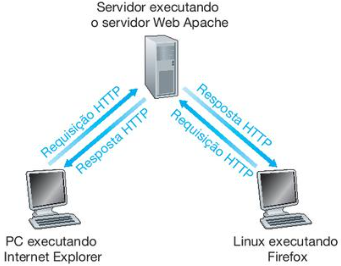
\includegraphics[scale=0.5]{figuras/figura04_01}}
\end{frame}

\begin{frame}{Descrição Geral}
    \begin{itemize}
        \justifying
        \item O HTTP utiliza o TCP como protocolo de transporte
            \begin{itemize}
                \justifying
                \item Portanto é uma aplicação cujas pontas criam uma conexão;
                \item Não precisa se preocupar como será feita a entrega de dados, ou sobre a garantia de entrega (trabalho do TCP).
            \end{itemize}
    \end{itemize}
\end{frame}

\begin{frame}{HTTP e conexões não persistentes}
    \begin{itemize}
        \justifying
        \item<1> Em uma \textbf{conexão não persistente} as mensagens entre cliente e servidor acontecem através de várias conexões distintas.
        \item<1> Entretanto, o HTTP tem como padrão a conexão persistente.
        \item<2-> EXEMPLO
            \begin{itemize}
                \footnotesize
                \item<2-> Suponha o acesso a uma página contendo 11 objetos: 1 arquivo HTML e 10 imagens. Suponha também que todos os objetos estão no mesmo servidor, cuja url é \url{http://www.exemplo.com/meuExemplo/home.index}. Vamos ver o passo-a-passo:
                \begin{enumerate}
                    \justifying
                    \tiny
                    \item<3-4> O processo cliente HTTP inicia uma conexão TCP para o servidor \url{www.exemplo.com} na porta 80 (associados à conexão TCP teremos um \textit{socket} no cliente e outro no servidor).
                    \item<4-5> O cliente envia uma mensagem de requisição HTTP ao servidor por meio do seu \textit{socket}. A mensagem inclui o nome do caminho, ou seja: \url{/meuExemplo/home.index}.
                    \item<5-6> O processo servidor HTTP recebe a mensagem pelo seu \textit{socket}, extrai de seu armazenamento o objeto pedido, e o envia através de seu \textit{socket} como uma mensagem de resposta.
                    \item<6-7> O processo servidor ordena ao TCP que a conexão seja encerrada (o TCP vai encerrar somente quando tiver certeza de que o cliente recebeu a mensagem de resposta intacta).
                    \item<7-8> O cliente HTTP recebe a mensagem, e a conexão TCP é encerrada. A mensagem é um arquivo HTML, o qual contem referências às dez imagens.
                    \item<8> Os passos 1 - 4 são repetidos para cada imagem referenciada.
                \end{enumerate}
            \end{itemize}
    \end{itemize}
\end{frame}

\begin{frame}{HTTP e conexões não persistentes}
    \centering
    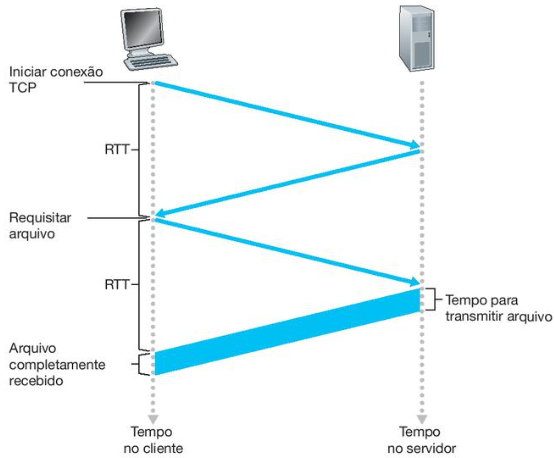
\includegraphics[scale=0.6]{figuras/figura04_02}
\end{frame}

\begin{frame}{HTTP e conexões persistentes}
    \begin{itemize}
        \justifying
        \item Conexões não persistentes possuem algumas desvantagens
            \begin{itemize}
                \justifying
                \item A necessidade de uma conexão para cada troca de mensagem pode sobrecarregar o servidor.
                \item O carregamento de vários objetos leva mais tempo.
            \end{itemize}
        \item<2-> Em conexões persistentes vários objetos e mensagens podem ser transferidos em uma única conexão (ex.: várias páginas em um mesmo site).
        \item<3-> As requisições em uma conexão persistente podem ser feitas mesmo antes de chegar a resposta para requisições pendentes (paralelismo $\rightarrow$ padrão no HTTP). Desta forma, a transferência pode ocorrer de forma ininterrupta.
        \item<4> Um servidor HTTP encerra uma conexão quando deixa de ser usada por algum tempo (configurável).
    \end{itemize}
\end{frame}

\begin{frame}{Mensagem de requisição}
    \centering
    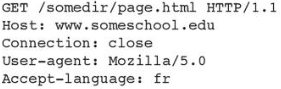
\includegraphics[scale=0.7]{figuras/figura04_03}
    \begin{itemize}
        \justifying
        \item Essa mensagem tem 5 linhas (porém é possível ter mais linhas, ou menos também).
        \item \textbf{linha de requisição}: a primeira linha. Possui três campos: \textit{método}, \textit{url} e \textit{versão} do HTTP. Outros métodos possíveis são POST, HEAD, PUT e DELETE.
        \item \textbf{linhas de cabeçalho}: as demais 4 linhas.
            \begin{enumerate}
                \justifying
                \item Especifica o hospedeiro onde está o objeto (essa é uma informação exigida pelo \textit{proxy}).
                \item Indica que a conexão deverá ser não persistente.
                \item Especifica o agente de usuário (o navegador) utilizado.
                \item Indica que o usuário prefere receber uma versão em Francês do objeto. Caso não exista, o servidor retornará com a versão \textit{default}.
            \end{enumerate}
    \end{itemize}
\end{frame}

\begin{frame}{Mensagem de requisição}
    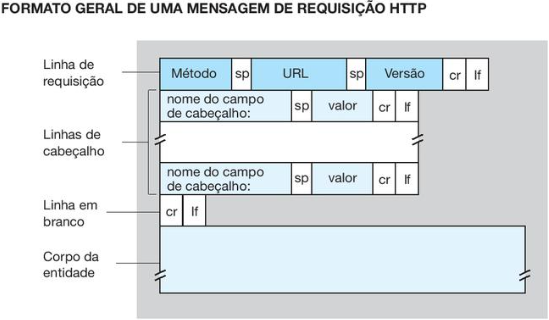
\includegraphics[scale=0.7]{figuras/figura04_04}
\end{frame}

\begin{frame}{Mensagem de resposta}
    \centering
    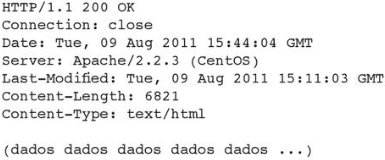
\includegraphics[scale=0.6]{figuras/figura04_05}
    \begin{itemize}
        \justifying
        \item Três seções: \textbf{linha de estado}, \textbf{linhas de cabeçalho} e \textbf{corpo da entidade}.
        \item \textbf{linha de estado}: três campos $\rightarrow$ versão do protocolo, código de estado e mensagem de estado correspondente.
        \item \textbf{linhas de cabeçalho}
            \begin{enumerate}
                \justifying
                \item O servidor informa que encerrará a conexão TCP após o envio da mensagem.
                \item Indica a data e hora em que a resposta foi criada e enviada.
                \item Mostra que a mensagem foi gerada por um servidor Apache.
                \item Indica a data e hora em que o objeto foi criado, ou sua última modificação.
                \item Indica o número de bytes do objeto que está sendo enviado.
                \item Mostra o tipo do objeto (neste caso um text/html).
            \end{enumerate}
    \end{itemize}
\end{frame}

\begin{frame}{Mensagem de resposta}
    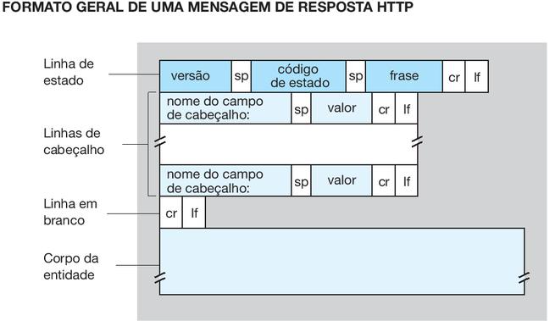
\includegraphics[scale=0.7]{figuras/figura04_06}
\end{frame}

\begin{frame}{}
    \centering
    \Large
    SMTP
\end{frame}

\begin{frame}{Descrição Geral}
    \begin{itemize}
        \justifying
        \item \textit{Simple Mail Transfer Protocol}
        \item É o principal protocolo da camada de aplicação do correio eletrônico da Internet.
        \item Utiliza o TCP como protocolo de transporte.
        \item É mais antigo que o HTTP. Sua idade é perceptível pelas suas restrições (ex.: para os nossos tempos seu limite de dados é muito pequeno).
    \end{itemize}
\end{frame}

\begin{frame}{Descrição Geral}
    \centering
    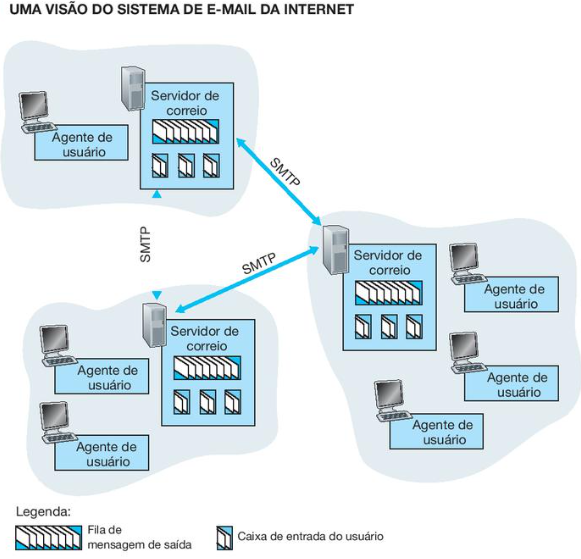
\includegraphics[scale=0.5]{figuras/figura04_07}
\end{frame}

\begin{frame}{Exemplo}
    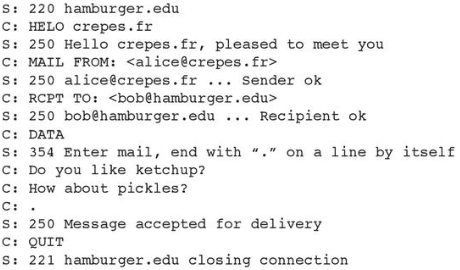
\includegraphics[scale=0.8]{figuras/figura04_08}
\end{frame}

\begin{frame}{}
    \centering
    \Large
    DNS
\end{frame}

\begin{frame}{Descrição Geral}
    \begin{itemize}
        \justifying
        \item \textit{Domain Name System}
        \item É um banco de dados distribuído, executado em uma hierarquia de \textbf{servidores de DNS} e também um protocolo da camada de aplicação (o qual permite que hospedeiros consultem o banco de dados distribuído).
        \item Utiliza o UDP como procolo da camada de transporte, e a porta 53.
        \item É utilizado também pelos outros protocolos da camada de aplicação (isso mesmo, o HTTP e SMTP, por exemplo).
    \end{itemize}
\end{frame}

\begin{frame}{Como funciona}
    \begin{itemize}
        \justifying
        \item A máquina do usuário executa o lado cliente do DNS.
        \item O navegador extrai o nome da URL e passa para o cliente DNS.
        \item O cliente DNS envia uma consulta com o nome do hospedeiro para um servidor DNS.
        \item O cliente DNS recebe uma resposta, incluindo o IP do hospedeiro.
        \item Outras aplicações (e protocolos) podem utilizar o IP para abrir uma conezão TCP.
    \end{itemize}
\end{frame}

\begin{frame}{Outros serviços}
    \begin{itemize}
        \justifying
        \item<1> \textbf{Apelidos (\textit{aliasing})}: um hospedeiro pode ter um ou mais apelidos. Nesses casos até mesmo o \textbf{nome canônico} é difícil de decorar. O DNS pode fornecer o nome canônico associado a algum apelido, e também o IP.
        \item<2> \textbf{Apelidos de servidor de correio}: imagine o email aluno@estacio.com; apesar de simples, o nome canônico do \textit{estacio.com} pode ser mais complicado. O DNS também fornece o nome canônico e IP de um servidor de email.
        \item<3> \textbf{Distribuição de carga}: alguns servidores são replicados, ou seja, o mesmo conteúdo está presente em mais de um servidor, cada um com seu IP. O DNS guarda o conjunto de IPs relacionado ao nome e passa para o cliente. No lado cliente o DNS faz um rodízio da ordem deles e, na prática, distribui a carga de requisições.
    \end{itemize}
\end{frame}

\begin{frame}{Escalabilidade}
    \begin{itemize}
        \justifying
        \item O DNS utiliza um grande número de servidores, organizados de maneira hierárquica, por isso, nenhum servidor terá, em si, todos os mapeamentos para todos os IPs.
        \item Três classes de servidores: raiz, de domnínio de alto nível (\textit{top-level domain} - TLD) e autoritativos.
        \item \textbf{Servidores Raiz}: 13 servidores (denominados de A a M). Cada servidor destes pode ser um conjunto de servidores replicados (redundância).
        \item<2-> \textbf{Servidores de Domínio de Alto Nível}: responsáveis por domínios como \textit{com}, \textit{org}, \textit{net}, \textit{edu}, \textit{gov} e os de alto níveis de cada país, por exemplo \textit{br}.
        \item<3-> \textbf{Servidores Autoritativos}: servidores de organizações (universidades e empresas de grande porte) que possuem hospedeiros que podem ser acessados publicamente.
        \item<4-> Ainda existem também os servidores locais, os quais não fazer parte, estritamente, da hierarquia.
    \end{itemize}
\end{frame}

\begin{frame}{Escalabilidade}
    \centering
    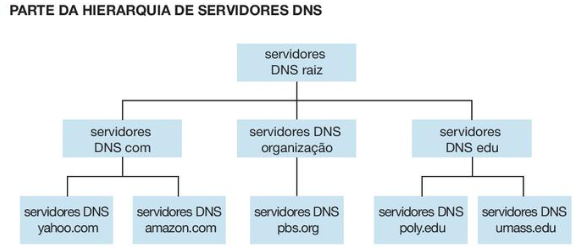
\includegraphics[scale=0.7]{figuras/figura04_09}
\end{frame}

\begin{frame}{Escalabilidade}
    \centering
    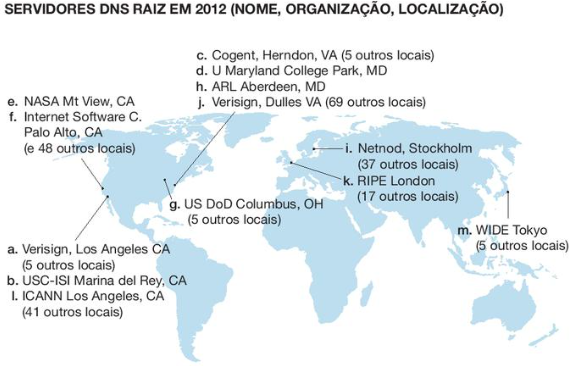
\includegraphics[scale=0.7]{figuras/figura04_10}
\end{frame}

%=============================================================================
% SECTION 4
%=============================================================================
\section{Camada de Transporte}

%-----------------------------------------------------------------------------
% SUBSECTION 4.1
%-----------------------------------------------------------------------------
\subsection{Serviços de transporte disponíveis para aplicações}

\begin{frame}{}
    \centering
    \Large
    Camada de Transporte\\
    \large
    Serviços de transporte disponíveis para aplicações
\end{frame}

\begin{frame}{Serviços de transportes para aplicações}
    \begin{itemize}
        \justifying
        \item Transferência confiável de dados
            \begin{itemize}
                \justifying
                \item<1> Uma aplicação \textit{sensível} (e-mail, transferência de arquivo, movimentação financeira, etc.) deve utilizar um protocolo que garanta a transferência confiável dos dados. A perda de dados para essas aplicações podem ser catastróficas.
                \item<1> Aplicações \textbf{tolerantes a perda} são pouco afetados se algumas informações não chegam ao destino.
            \end{itemize}
        \item<2-> Vazão
            \begin{itemize}
                \justifying
                \item<2> Vazão é a taxa pela qual o processo remetente pode enviar bits ao destinatário.
                \item<2> A vazão pode ser variável ao longo do tempo (outras aplicações enviando e recebendo dados). Um protocolo pode garantir uma vazão a uma taxa específica.
                \item<2> Uma aplicação pode solicitar uma vazão garantida e o protocolo vai garantir, no mínimo, a vazão solicitada.
                \item<2> Aplicações que possuem necessidae de vazão são conhecidas como \textbf{sensíveis à largura de banda}.
            \end{itemize}
    \end{itemize}
\end{frame}

\begin{frame}{Serviços de transportes para aplicações}
    \begin{itemize}
        \justifying
        \item Temporização
            \begin{itemize}
                \justifying
                \item<1> Serviço que garante um tempo máximo para a entrega dos dados.
                \item<1> Exemplos: MS Teams, jogos online, etc.
            \end{itemize}
        \item<2> Segurança
            \begin{itemize}
                \justifying
                \item<2> Uma aplicação pode necessitar de segurança para a transferência dos dados.
                \item<2> Um protocolo pode fornecer sigilo entre dois processos/usuários ao codificar a mensagem antes de ser enviada.
            \end{itemize}
    \end{itemize}
\end{frame}

\begin{frame}{Serviços de transportes para aplicações}
    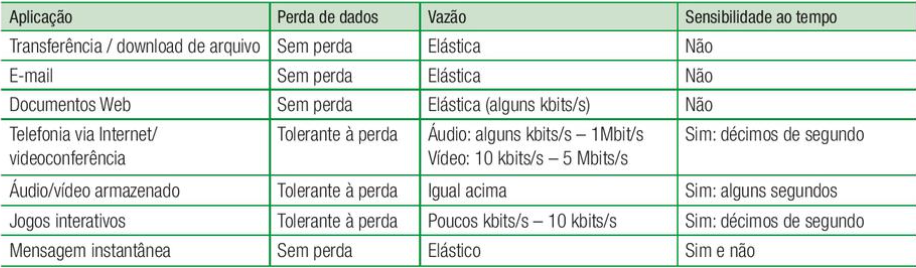
\includegraphics[width=\textwidth]{figuras/figura03_01}
\end{frame}

%-----------------------------------------------------------------------------
% SUBSECTION 4.2
%-----------------------------------------------------------------------------
\subsection{Serviços providos pela Internet}

\begin{frame}{}
    \centering
    \Large
    Camada de Transporte\\
    \large
    Serviços providos pela Internet
\end{frame}

\begin{frame}{Serviços providos pela Internet}
    \begin{itemize}
        \justifying
        \item A Internet (TCP/IP) disponibiliza dois protocolos de transporte para aplicações: TCP e UDP. Cada protocolo oferece um conjunto diferente de serviços.
        \item TCP
            \begin{itemize}
                \justifying
                \item<2> É orientado para conexão e confiabilidade de transferência de dados.
                \item<2> \textbf{Conexão}: o TCP faz cliente e servidor trocarem informações de controle de cama de transporte \alert<2>{antes} que as mensagens da camada de aplicação comecem a fluir.
                \item<2> \textbf{Transporte}: o TCP garante a entrega de todos os dados sem erro e na ordem correta, e também sem duplicação.
                \item<2> Além disso, o TCP também faz o controle de congestionamento.
            \end{itemize}
        \item UDP
            \begin{itemize}
                \justifying
                \item<3> É um protocolo simplificado e leve. Não garante a transferência confiável de dados, a ordem correta de chegada e nem o controle de tráfego.
            \end{itemize}
        \item<4> Nenhum dos protocolos de transporte da internet provê serviço de vazão e temporização. As aplicações lidam de forma inteligente com essas limitações.
    \end{itemize}
\end{frame}

\begin{frame}{Serviços providos pela Internet}
    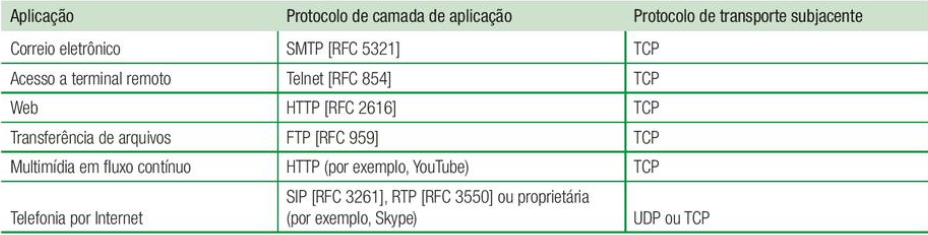
\includegraphics[width=\textwidth]{figuras/figura03_02}
\end{frame}

%-----------------------------------------------------------------------------
% SUBSECTION 4.3
%-----------------------------------------------------------------------------
\subsection{UDP}

\begin{frame}{}
    \centering
    \Large
    UDP
\end{frame}

\begin{frame}{UDP}
    \begin{itemize}
        \justifying
        \item Definido no RFC 768;
        \item É um protocolo não orientado a conexão;
        \item Basicamente seu funcionamento é pegar mensagens do processo da aplicação, anexar os campos de número da porta de origem e de destino para o \alert<2>{serviço de multiplexação/demultiplexação}, adicionar dois outros pequenos campos e passar o segmento resultante para a camada rede.
    \end{itemize}
\end{frame}

\begin{frame}{UDP}
    \begin{itemize}
        \item Estrutura do Segmento UDP\\
        \centering
        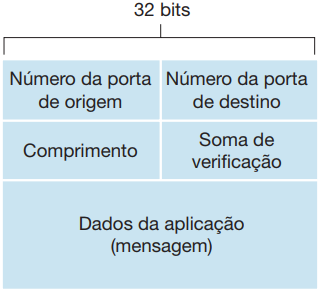
\includegraphics[width=0.6\textwidth]{figuras/figura06_02}
    \end{itemize}
\end{frame}

\begin{frame}{UDP}
    \begin{itemize}
        \justifying
        \item \textbf{Soma de verificação} (\textit{checksum}): serve para o UDP detectar se algum bit do segmento foi alterado. É opcional.
        \item \textbf{Como funciona}: no remetente todas as palavras de 16 bits são somadas. Ao fim da soma, teremos um resultado. O complemento deste resultado é a soma de verificação. No destinatário todas as palavras são somadas novamente, desta vez acrescentando a soma de verificação. O resultado deve ser 1111111111111111 (16 bits 1). Se houver qualquer bit 0, há um erro no segmento.
        \item Existem ainda mais detalhes que podem ser visualizados nos RFCs, ou no livro do Frouzan (a partir da página 712).
    \end{itemize}
\end{frame}

%-----------------------------------------------------------------------------
% SUBSECTION 4.4
%-----------------------------------------------------------------------------
\subsection{TCP}

\begin{frame}{}
    \centering
    \Large
    TCP
\end{frame}

\begin{frame}{TCP}
    \begin{itemize}
        \justifying
        \item É orientado a conexão (\textbf{ponto a ponto});
        \item Provê um serviço \textbf{\textit{full-duplex}}, ou seja, os dados de remetente e destinatário podem fluir ao mesmo tempo. Também é um s
        \item A conexão é feita através de uma apresentação de três vias, ou \textit{3-way handshake}, ou seja, o cliente inicia enviando ao servidor um segmento TCP especial. O servidor responde com outro segmento TCP especial e, por fim, o cliente responde com um terceiro segmento especial. Neste ponto os parâmetros para transferência de dados são estabelecidos.
    \end{itemize}
\end{frame}

\begin{frame}{TCP}
    \begin{itemize}
        \justifying
        \item Estabelecida a conexão, o TCP recebe a mensagem vinda do \textit{socket} e o repassa ao \textbf{buffer de envio}, onde será dividido em partes menores, chamados segmentos, os quais são passados para a camada de rede.
        \item A \textbf{unidade máxima de transmissão} (MTU --- \textit{Maximum transmission unit}) é o valor do maior quadro de enlace que pode ser enviado pelo remetente. A partir desse valor é possível calcular o MSS (\textit{Maximum Segment Size}), ou \textbf{tamanho máximo do segmento}, ou seja, a quantidade máxima de dados da camada de aplicação que cabem no segmento de forma que, junto com o cabeçalho do TCP, o segmento inteiro caiba no quadro.
    \end{itemize}
\end{frame}

\begin{frame}{TCP}
    \begin{itemize}
        \item Estrutura do segmento TCP\\
        \centering
        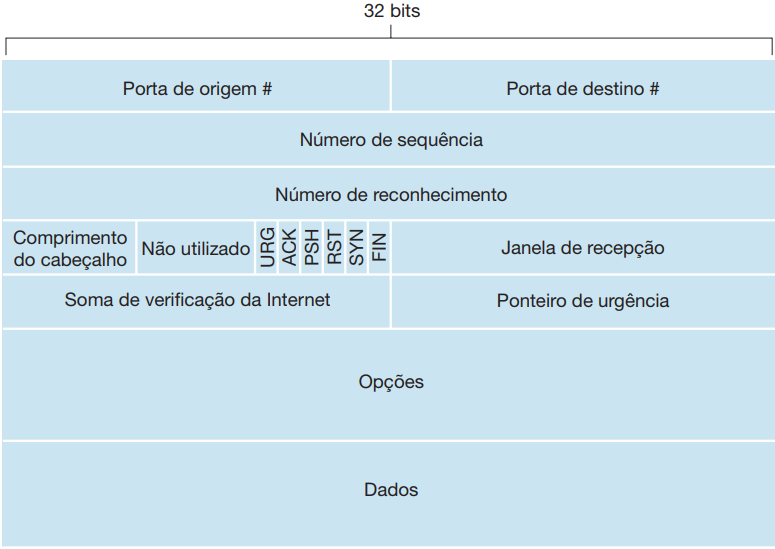
\includegraphics[scale=0.48]{figuras/figura06_03}
    \end{itemize}
\end{frame}

\begin{frame}{TCP}
    \begin{itemize}
        \justifying
        \item \textbf{Porta de destino/origem}: valor da porta utilizada pelo processo de aplicação.
        \item \textbf{Número de sequência} e \textbf{de reconhecimento}: números (de 32 bits cada) utilizados pelo TCP  para o serviço confiável de transferência de dados.
        \item \textbf{Janela de recepção}: 16 bits usados para controle de fluxo. Indica o número de bytes que um destinatário está disposto a aceitar.
        \item \textbf{Comprimento do cabeçalho}: 4 bits que especificam o comprimento do cabeçalho TCP em palavras de 32 bits.
        \item \textbf{Soma de verificação}: análogo ao \textit{checksum} do UDP.
    \end{itemize}
\end{frame}

\begin{frame}{TCP}
    \begin{itemize}
        \justifying
        \item \textbf{Opções}: opcional e de comprimento variável. Usado quando remetente e destinatário negociam o MSS, ou como um fator de aumento de escala da janela para utilização em redes de alta velocidade.
        \item \textbf{Flag}: 6 bits:
            \begin{itemize}
                \justifying
                \item \textbf{ACK}: Indica se o segmento contém um reconhecimento para um segmento que foi recebido com sucesso.
                \item \textbf{RST}, \textbf{SYN} e \textbf{FIN}: usados para estabelecer e encerrar uma conexão.
                \item \textbf{PSH}: indica que o destinatário deve passar os dados para a camada superior imediatamente.
                \item \textbf{URG}: indica que há dados nesse segmento que a entidade da camada superior do remetente marcou como urgente. A localização do último byte dos dados urgentes é indicado no campo \textbf{Ponteiro de urgência}.
            \end{itemize}
    \end{itemize}
\end{frame}

%=============================================================================
% SECTION 4
%=============================================================================
\section{Camada de Rede}

%-----------------------------------------------------------------------------
% SUBSECTION 4.4
%-----------------------------------------------------------------------------
\subsection{IP}

\begin{frame}{}
    \centering
    \Large
    Camada de Rede\\
    \large
    Internet Protocol (IP)
\end{frame}

\begin{frame}{IP}
    \begin{itemize}
        \justifying
        \item Um \textbf{endereço IPv4} é um endereço de 32 bits.
        \item $2^{32} = 4.294.967.296$ valores possíveis.
        \item Duas notações: \textbf{binária} e \textbf{decimal pontuada}.
            \begin{itemize}
                \item 01110101 10010101 00011101 00000010
                \item 117.149.29.2
            \end{itemize}
        \item De início o IPv4 usava o \textbf{endereçamento com classes}: A, B, C, D e E.
    \end{itemize}
    \centering
    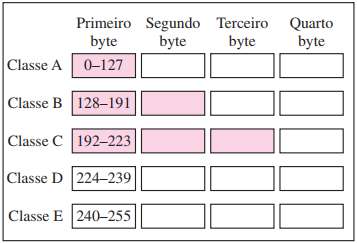
\includegraphics[scale=0.7]{figuras/figura06_04}
\end{frame}

\begin{frame}{IP}
    \centering
    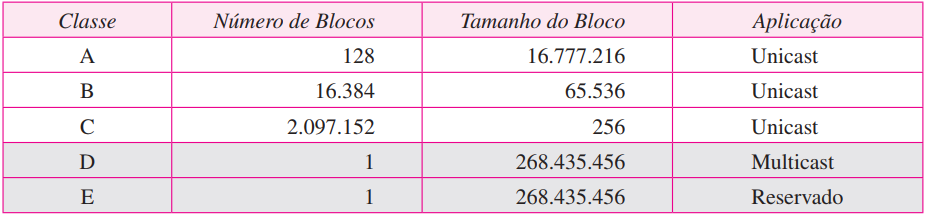
\includegraphics[scale=0.45]{figuras/figura06_05}
\end{frame}

\begin{frame}{IP}
    \begin{itemize}
        \justifying
        \item \textbf{Endereços classe A}: eram designados a grandes organizações com um grande número de hosts ou roteadores conectados.
        \item \textbf{Endereços classe B}: destinavam-se às organizações de médio porte com dezenas de milhares de hosts ou roteadores conectados.
        \item \textbf{Endereços classe C}: destinavam-se a pequenas organizações com um pequeno número de hosts ou roteadores.
        \item \textbf{Endereços classe D}: foram projetados para multicast. Cada endereço nessa classe é usado para definir um grupo de hosts.
        \item \textbf{Endereços classe E}: reservados para uso futuro.
        \vspace{1cm}
        \item Muitos endereços eram desperdiçados!
    \end{itemize}
\end{frame}

\begin{frame}{IP}
    \begin{itemize}
        \justifying
        \item \textbf{Netid} e \textbf{Hostid}
            \begin{itemize}
                \justifying
                \item No endereçamento com classe, os tipos A, B e C são divididos em netid e hostid.
                \item Classe A: 1 byte para netid e 3 bytes para hostid.
                \item Classe B: 2 bytes para netid e 2 bytes para hostid.
                \item Classe C: 3 bytes para netid e 1 byte para hostid.
            \end{itemize}
        \item Esgotamento de endereços
            \begin{itemize}
                \justifying
                \item Dado o tempo, a quantidade de endereços das classes A e B acabaram. Enquanto isso, um bloco de endereços C é muito pequeno para a maioria das organizações de porte médio.
                \item<2> Solução: endereçamento sem classes.
            \end{itemize}
    \end{itemize}
\end{frame}

\begin{frame}{Endereçamento sem Classes}
    \begin{itemize}
        \justifying
        \item Quando uma entidade precisa ser conectada à Internet, um bloco de endereços é concedido. 
        \item O tamanho do bloco é variável.
        \item Restrições:
            \begin{itemize}
                \item Os endereços em um bloco devem ser contíguos.
                \item O número de endereços deve ser uma potência de 2.
                \item O primeiro endereço tem de ser igualmente divisível pelo número de endereços.\\
                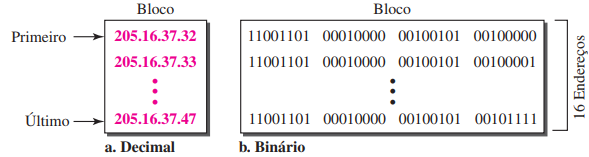
\includegraphics[scale=0.6]{figuras/figura06_06}
            \end{itemize}
        \item No exemplo os endereços são contíguos (205.16.37.32 ... 205.16.37.47). A quantidade de enderços (16) é potência de 2. O primeiro endereço em binário, quando convertido em decimal é divisível por 16.
    \end{itemize}
\end{frame}

\begin{frame}{Endereçamento sem Classes}
    \begin{itemize}
        \justifying
        \item \textbf{Máscara}
            \begin{itemize}
                \justifying
                \item Usado para definir um bloco de endereços.
                \item É um número de 32 bits, no qual os $n$ números mais à esquerda sao 1, e os 32 - $n$ números mais à direita são 0.
                \item Notação: x.y.z.t/$n$, onde x.y.z.t define um dos endereços e /$n$ estipula a máscara.
            \end{itemize}
        \item \textbf{Primeiro endereço}: Os 32 - $n$ bits mais à direita são configurados como 0.
        \item \textbf{Último endereço}: Os 32 - $n$ bits mais à direita são configurados como 1.
    \end{itemize}
\end{frame}

\begin{frame}{Endereçamento sem Classes}
    \begin{itemize}
        \item Exemplo:
            \begin{itemize}
                \justifying
                \item Um dos endereços é 205.16.37.39/28. Como saber o primeiro endereço no bloco?
                \item O endereço em binário é\\ 
                \vspace{0.1 cm}
                11001101 00010000 00100101 00100111\\ 
                \vspace{0.1 cm}
                Se configurarmos os 32 - $n$ (32 - 28 neste caso) bits mais à direito como 0, teremos\\
                \vspace{0.1 cm}
                11001101 00010000 00100101 001\textbf{0000}\\ 
                \vspace{0.1 cm}
                que em decimal é 205.16.37.32.
                \item Como encontrar o último endereço? Em vez 0, configuramos como 1:\\ 
                \vspace{0.1 cm}
                11001101 00010000 00100101 0010\textbf{1111}\\ 
                \vspace{0.1 cm}
                o que dá 205.16.37.47.
                \item O número de endereços pode ser calculado como $2^{32 - n} = 2^{32 - 28} = 2^{4} = 16$.
            \end{itemize}
    \end{itemize}
\end{frame}

\begin{frame}{Endereçamento sem Classes}
    \begin{itemize}
        \justifying
        \item Outra forma é utilizar a máscara inteira. Ou seja, quando $n = 28$ isso significa que a máscara é: \\
        \vspace{0.1 cm}
        11111111 11111111 11111111 11110000
        \item O primeiro endereço é descobertao ao ser aplicar o \textbf{AND} entre o endereço fornecido e a máscara.
        \item O último endereço é obtido aplicando o \textbf{OR} com o endereço fornecido e o complemento da máscara, ou seja:\\
        \vspace{0.1cm}
        00000000 00000000 00000000 00001111
        \item A quantidade de endereços é o valor decimal do complemento da máscara + 1. No nosso caso, os quatro últimos bits são 1111. Então temos $2^{0} + 2^{1} + 2^{2} + 2^{3} = 1 + 2 + 4 + 8 = 15$. Adicionado 1 a 15 temos 16 endereços no bloco.
    \end{itemize}
\end{frame}

\begin{frame}{Endereços de Rede}
    \begin{itemize}
        \justifying
        \item Quando uma organização recebe um bloco de endereços IP, o primeiro deles é o endereço da rede (comumente, mas nem sempre).
        \item O endereço da rede é o que estabelece a organização para o restante do mundo.
        \item Exemplo: configuração de rede para o bloco 205.16.37.32/28\\
        \centering
        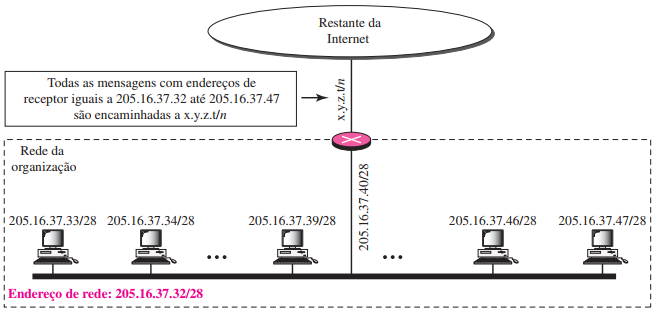
\includegraphics[scale=0.5]{figuras/figura09_01}
        \justifying
        \item A rede da organização é conectada à Internet por meio de um roteador, que tem dois endereços: um pertence ao bloco concedido; os demais pertencem à rede que se encontra do outro lado do roteador.
    \end{itemize}
\end{frame}

\begin{frame}{Hierarquia}
    \begin{itemize}
        \item Os endereços IP apresentam níveis de hierarquia.
        \item \textbf{Hierarquia de Dois Níveis} (sem o uso de sub-redes)
            \begin{itemize}
                \justifying
                \item Os $n$ bits mais à esquerda do endereço x.y.z.t/n designam a rede (\textbf{prefixo}).
                \item Os $32 - n$ bits mais à direita estabelecem o host particular (\textbf{sufixo}).\\
                %\centering
                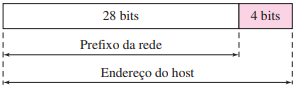
\includegraphics[scale=0.7]{figuras/figura09_02}
            \end{itemize}
    \end{itemize}
\end{frame}

\begin{frame}{Hierarquia}
    \begin{itemize}
        \item \textbf{Hierarquia de Três Níveis} (uso de sub-redes)
            \begin{itemize}
                \justifying
                \item<1> Quando alguma organização recebe uma grande quantidade de endereços, é possível que ela queira dividi-los em blocos menores (ou \textit{clusters}), as chamadas sub-redes.
                \item<1> A Internet enxerga apenas uma rede, porém internamente podem existir várias.
                \item<1> A mensagem chega ao roteador da rede, o qual envia a mensagem para o roteador da sub-rede.
                \item<2-> Exemplo: Supondo que uma empresa tenha recebido o bloco 17.12.40.0/26 com 64 endereços.\\ 
                A empresa tem 3 escritórios e decide dividir os endereços da seguinte forma: 32, 16, 16. As novas máscaras podem ser descobertas da seguinte forma:\\
                A primeira sub-rede terá 32 endereços então sua máscara n1 tem de ser igual a 27 ($32 - 27 = 5 \therefore 2^{5} = 32$).\\
                Como as outras duas sub-redes terão 16 endereços, então n2 = n3 = 28.\\
                Portanto temos as máscaras 27, 28 e 28 com a máscara da empresa sendo 26.
            \end{itemize}
    \end{itemize}
\end{frame}

\begin{frame}{Hierarquia}
    \centering
    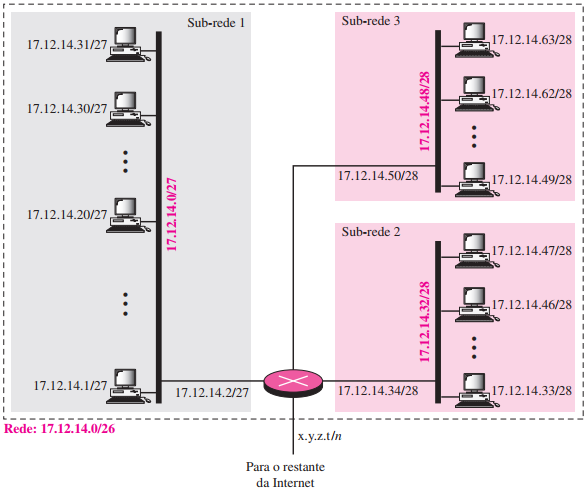
\includegraphics[scale=0.5]{figuras/figura09_03}
\end{frame}

\begin{frame}{Hierarquia}
    \begin{itemize}
        \tiny
        \justifying
        \item \textbf{Hierarquia de Três Níveis} (uso de sub-redes)
            \begin{itemize}
                \tiny
                \justifying
                \item Descobrindo os endereços \textbf{de} sub-rede a partir de um dos endereços \textbf{na} sub-rede.\\
                Na sub-rede 1, o endereço 17.12.14.29/27 nos fornece o endereço de sub-rede quando aplicamos a máscara /27
                \begin{exampleblock}{17.12.14.29/27}
                    \begin{tabular}{l l}
                        \tiny
                        Host:       &  00010001 00001100 00001110 000\textbf{11101}\\
                        Máscara:    & /27\\
                        Sub-rede:   & 00010001 00001100 00001110 00000000 $\rightarrow$ 17.12.14.0
                    \end{tabular}
                \end{exampleblock}
                Na sub-rede 2, o endereço 17.12.14.45/28 nos fornece o endereço de sub-rede quando aplicamos a máscara /28
                \begin{exampleblock}{17.12.14.45/28}
                    \begin{tabular}{l l}
                        \tiny
                        Host:       &  00010001 00001100 00001110 0010\textbf{1101}\\
                        Máscara:    & /28\\
                        Sub-rede:   & 00010001 00001100 00001110 00100000 $\rightarrow$ 17.12.14.32
                    \end{tabular}
                \end{exampleblock}
                Na sub-rede 3, o endereço 17.12.14.50/28 nos fornece o endereço de sub-rede quando aplicamos a máscara /28
                \begin{exampleblock}{17.12.14.50/28}
                    \begin{tabular}{l l}
                        \tiny
                        Host:       &  00010001 00001100 00001110 0011\textbf{0010}\\
                        Máscara:    & /28\\
                        Sub-rede:   & 00010001 00001100 00001110 00110000 $\rightarrow$ 17.12.14.48
                    \end{tabular}
                \end{exampleblock}
            \end{itemize}
    \end{itemize}
\end{frame}

\begin{frame}{Hierarquia}
    \begin{itemize}
        \item \textbf{Hierarquia de Três Níveis} (uso de sub-redes)\\
        \centering
        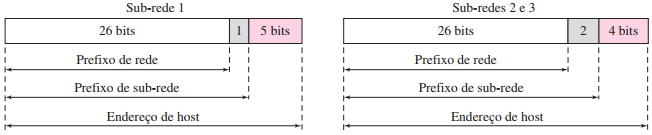
\includegraphics[width=0.9\textwidth]{figuras/figura09_04}
        \justifying
        \item A estrutura de endereçamento sem classes não restringe o número de níveis hierárquicos.
        \item Uma organização pode dividir o bloco de endereços concedido em sub-blocos.
        \item Cada sub-bloco pode, por seu lado, ser dividido em sub-blocos menores, e assim por diante.
    \end{itemize}
\end{frame}

\begin{frame}{Alocação de Endereços}
    \begin{itemize}
        \justifying
        \item<1> ICANN (\textit{Internet Corporation for Assigned Names and Numbers}) ou \textit{Corporação da Internet para Nomes e Números Designados} é a responsável por alocar os endereços.
        \item<1> Normalmente a ICANN concede grandes blocos de endeços a ISPs, as quais fornecem seus serviços às empresas e usuários finais.
        \item<2-> Exemplo: Um ISP recebe um bloco de endereços iniciando em 190.100.0.0/16 (65.536 endereços). Esse ISP precisa distribuir esses endereços para três grupos de clientes, como segue:
            \begin{enumerate}[a)]
                \justifying
                \item<2-> O primeiro grupo apresenta 64 clientes; cada um deles precisa de 256 endereços.
                \item<2-> O segundo grupo tem 128 clientes; cada um deles precisa de 128 endereços.
                \item<2-> O terceiro grupo contém 128 clientes; cada um deles precisa de 64 endereços.
            \end{enumerate}
    \end{itemize}
\end{frame}

\begin{frame}{Alocação de Endereços}
    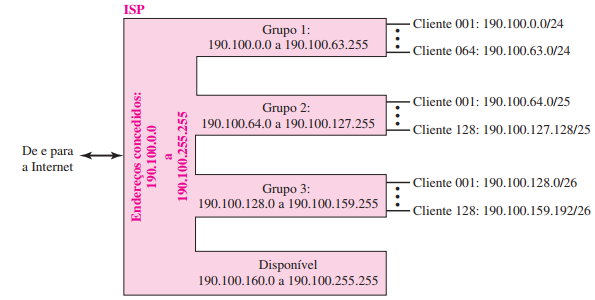
\includegraphics[scale=0.68]{figuras/figura09_05}
\end{frame}

%=============================================================================
% SECTION REFERENCES
%=============================================================================
%\begin{frame}[allowframebreaks]{Referências}
%    \scriptsize
%    \printbibliography
%\end{frame}

\end{document}













%% ---------------------------------------------------------------------------
% This presentation is separated by sections and subsections
%\section{Seção I}
%\begin{frame}{Explicações}
%    % itemize
%    Este é um template que pode ser utilizado para:
%    \begin{itemize}
%        \item Apresentação de Trabalhos Acadêmicos
%        \item Apresentação de Disciplinas
%        \item Apresentações de Teses e Dissertações
%    \end{itemize}
%
%    \vspace{0.4cm} % vertical space
%    
%    % enumeration
%    Para utilizar este template corretamente é importante que:
%    \begin{enumerate}
%        \item Tenha conhecimento mínimo sobre LaTeX
%        \item Ler os comentários no template (explicações)
%        \item Ler o README.md (documentação)
%    \end{enumerate}
%
%    \vspace{0.2cm}

%    \example{Este é um texto de exemplo!} \emph{Texto de Ênfase!}
%\end{frame}

%% ---------------------------------------------------------------------------
%\subsection{Subseção I}
%\begin{frame}{Criando Blocos}
%    % Blocks styles
%    \begin{block}{Bloco Padrão}
%        Texto do corpo do bloco.
%    \end{block}

%    \begin{alertblock}{Bloco de Alerta}
%        Texto do corpo do bloco.
%    \end{alertblock}
%
%    \begin{exampleblock}{Bloco de Exemplo}
%        Texto do corpo do bloco.
%    \end{exampleblock}   
%\end{frame}

%% ---------------------------------------------------------------------------
%\subsection{Subseção II}
%\begin{frame}{Criando Caixas}
%    \successbox{testando o success box}
%
%    \pause
%
%    \alertbox{testando o alert box}
%
%    \pause
%
%    \simplebox{testando o simple box}
%\end{frame}

%% ---------------------------------------------------------------------------
%\subsection{Subseção III}
%\begin{frame}{Criando Algoritmos (Pseudocódigo)}
%    \begin{algorithm}[H]
%        \SetAlgoLined
%        \LinesNumbered
%        \SetKwInOut{Input}{input}
%        \SetKwInOut{Output}{output}
%        \Input{x: float, y: float}
%        \Output{r: float}
%        \While{True}{
%          r = x + y\;
%          \eIf{r >= 30}{
%           ``O valor de $r$ é maior ou iqual a 10.''\;
%           break\;
%           }{
%           ``O valor de $r$ = '', r\;
%          }
%         } 
%         \caption{Algorithm Example}
%    \end{algorithm}
%\end{frame}

%% ---------------------------------------------------------------------------

%\begin{frame}{Inserindo Algoritmos}
%    \lstset{language=Python}
%    \lstinputlisting[language=Python]{code/main.py}
%\end{frame}

%% ---------------------------------------------------------------------------
%\begin{frame}{Inserindo Algoritmos}
%    \lstinputlisting[language=C]{code/source.c}
%\end{frame}

%% ---------------------------------------------------------------------------
%\begin{frame}{Inserindo Algoritmos}
%    \lstinputlisting[language=Java]{code/helloworld.java}
%\end{frame}

%% ---------------------------------------------------------------------------
%\begin{frame}{Inserindo Algoritmos}
%    \lstinputlisting[language=HTML]{code/index.html}
%\end{frame}

%% ---------------------------------------------------------------------------
% This frame show an example to insert multicolumns
%\section{Multicolunas}
%\begin{frame}{Seção II - Multicolunas}
%    \begin{columns}{}
%        \begin{column}{0.5\textwidth}
%            \justify
%            É possível colocar mais de uma coluna utilizando os comandos de $\backslash$begin\{column\}\{\} e $\backslash$end\{column\}
%        \end{column}
%        \begin{column}{0.5\textwidth}
%            \justify
%            Porém, o espaçamento deve ser proporcional entre as colunas para que estas colunas não entrem em coflito. O espaçamento é dado pelo segundo argumento do $\backslash$begin.
%        \end{column}
%    \end{columns}    
%\end{frame}

%% ---------------------------------------------------------------------------
% This frame show an example to insert figures
%\section{Imagens}
%\begin{frame}{Seção III - Figures}
%    \begin{figure}
%        \centering
%        \caption{Emblema da UFC.}
%        
\includegraphics[scale=0.3]{libs/emblemufc.pdf}
%        \source{Obtido pelo site oficial da UFC \cite{siteufc} \cite{einstein}}
%        \label{fig:ufc_emblem}
%    \end{figure}
%\end{frame}

%% ---------------------------------------------------------------------------
% Reference frames
%\begin{frame}[allowframebreaks]
%    \frametitle{Referências}
%    \printbibliography
%\end{frame}

%% ---------------------------------------------------------------------------
% Final frame
%\begin{frame}{}
%    \centering
%    \huge{\textbf{\example{Obrigado(a) pela Atenção!}}}
%    
%    \vspace{1cm}
%    
%    \Large{\textbf{Contato:}}
%    \newline
%    \vspace*{0.5cm}
%    \large{\email{usuario@dominio}}
%\end{frame}